\documentclass[runningheads]{llncs}

% Must pass table option to xcolor before eccv.sty loads it
\PassOptionsToPackage{table,dvipsnames}{xcolor}

% ---------------------------------------------------------------
% ECCV package
% TODO REVIEW: Insert your submission number below by replacing '*****'
% TODO FINAL: Comment out the following line for the camera-ready version
\usepackage[review,year=2026,ID=11932]{eccv}
% TODO FINAL: Un-comment the following line for the camera-ready version
%\usepackage{eccv}

% ---------------------------------------------------------------
% Other packages

\usepackage{eccvabbrv}
\usepackage{graphicx}
\usepackage{booktabs}
\usepackage[accsupp]{axessibility}

% Additional packages from our paper
%% Additional packages and commands for the paper.

% Colors for table cells
% xcolor is loaded by eccv.sty; table option is passed in main.tex
\usepackage{multirow}

\colorlet{mediumgray}{gray!60}
\colorlet{lightergray}{gray!20}
\definecolor{lightred}{RGB}{255,200,200}
\definecolor{lightgreen}{RGB}{200,255,200}
\definecolor{lightyellow}{RGB}{255,255,200}
\definecolor{lightgray}{RGB}{200,200,200}

% Inline annotations
\newcommand{\red}[1]{{\color{red}#1}}
\newcommand{\todo}[1]{{\color{red}#1}}
\newcommand{\TODO}[1]{\textbf{\color{red}[TODO: #1]}}

\usepackage{algorithm}
\usepackage{algorithmic}
\usepackage{placeins}   % \FloatBarrier for precise float placement


% ---------------------------------------------------------------
% Hyperref
% TODO FINAL: Comment out the following line for the camera-ready version
\usepackage[pagebackref,breaklinks,colorlinks,citecolor=eccvblue]{hyperref}
% TODO FINAL: Un-comment the following line for the camera-ready version
%\usepackage{hyperref}

% ---------------------------------------------------------------
% Stub labels for main-paper cross-references.
% These provide the display text that appears when \ref is used in
% supplement sections that reference main-paper equations, figures, or
% sections.  Update the numbers if the main paper layout changes.

% Main-paper equations
\makeatletter
\newcommand{\stublabel}[2]{%
  \begingroup
    \protected@edef\@currentlabel{#2}%
    \label{#1}%
  \endgroup
}
\makeatother

\begin{document}

% ---------------------------------------------------------------
\title{mmIR: Supplementary Material}

\titlerunning{mmIR: Supplementary Material}

% TODO FINAL: Replace with your author list
\author{First Author\inst{1} \and
Second Author\inst{1} \and
Third Author\inst{1}}

\authorrunning{F.~Author et al.}

% TODO FINAL: Replace with your institution
\institute{University, City, Country\\
\email{\{first,second,third\}@university.edu}}

% Skip \maketitle (llncs forces \newpage, wasting page 1).
% Typeset a minimal header manually so content flows immediately.
% Convention follows ECCV supplements: "Supplement: [Full Paper Title]"
{\centering
  {\Large\bfseries Supplementary Material for\\ mmIR: Frequency-Space Inverse Rendering\\ for 3D Millimeter-Wave Radar ADC Synthesis\par}
  \vspace{0.5em}
  {Anonymous ECCV 2026 Submission\par}
  \vspace{0.25em}
  {Paper ID \#11932\par}
  \vspace{1.5em}
}

% ---------------------------------------------------------------
% Table of contents for supplement navigation
% Left-aligned section header, compact entries, all on page 1.
\setcounter{tocdepth}{2}
\section*{Table of Contents}
\vspace{-0.5em}
\begingroup
\hypersetup{linkcolor=black}
\small
\makeatletter
\@starttoc{toc}
\makeatother
\endgroup
\vspace{1em}

% ---------------------------------------------------------------
% Create stub labels for main-paper cross-references.
% These ensure that \ref{...} calls in the supplement sections resolve
% to the correct equation/figure/section numbers from the main paper.
% Update these if main-paper numbering changes.

\stublabel{eq:radar_bistatic}{1}
\stublabel{eq:path_adc}{5}
\stublabel{eq:ra_loss}{8}
\stublabel{eq:bsdf_full}{6}
\stublabel{sec:optimization}{3.4}
\stublabel{fig:antenna_layouts}{3}
\stublabel{fig:3d_single_frame_comparison}{5}
\stublabel{tab:training_ra}{2}
\stublabel{tab:radar_transfer}{3}
\stublabel{tab:3d_occupancy}{4}
\stublabel{sec:3d_occupancy}{4.3}

% ---------------------------------------------------------------
% Supplement sections

\setcounter{section}{0}
\renewcommand{\thesection}{\Alph{section}}

\section{TDM MIMO FMCW Theory}
\label{sec:rationale}

This section provides the signal-processing foundations that underpin our differentiable renderer, included for readers whose background is primarily in rendering or vision rather than radar.
Sec.~\ref{sec:supp_fmcw} derives the FMCW beat signal that the renderer must synthesize per traced path.
Sec.~\ref{sec:supp_iq} explains IQ demodulation, which determines why the renderer outputs \emph{complex}-valued ADC samples.
Sec.~\ref{sec:tdm_mimo_imaging} shows how these ADC samples are transformed into the 2D range--azimuth and 3D range--azimuth--elevation images used in our training loss (Eq.~\ref{eq:ra_loss}) and evaluation metrics.
Sec.~\ref{sec:supp_mc_derivation}--\ref{sec:supp_power_to_adc} derive the Monte Carlo estimator (main paper Eq.~3) and the power-to-ADC conversion that closes the forward model.
Readers familiar with FMCW radar may skip directly to Sec.~\ref{sec:supp_implementation}.

\subsection{FMCW Formulation}
\label{sec:supp_fmcw}

We summarize the standard FMCW signal model following~\cite{skolnik2001introduction,dudek2010millimeter}. FMCW radars emit a linearly frequency-modulated chirp into the scene,
\begin{equation}
    s(t) = A_s \cos\!\left(2\pi f_c t + \pi K t^2 \right), 
\end{equation}
for $\qquad 0 < t < T_c,$ and receive a delayed echo
\begin{equation}
    u(t) = A_r \cos\!\left(2\pi f_c (t-\tau) + \pi K (t-\tau)^2 \right), 
\end{equation}
for $\qquad \tau < t < T_c$, where $K$ is the chirp slope, $f_c$ is the start frequency, $T_c$ is the chirp duration, and $\tau = 2 d(t)/c$ is the round-trip delay for a target at range $d$ and wave propagation speed $c$. The total swept bandwidth is
\begin{equation}
    B = f_{\max} - f_{\min} = (f_c + K T_c) - f_c = K T_c.
\end{equation}

When the received chirp is mixed with the (still transmitting) chirp and low-pass filtered, the resulting real-valued beat signal is
\begin{equation}
    m_{\mathrm{R}}(t) \approx A_m 
    \cos\!\left(2\pi K \tau\, t + 2\pi f_c \tau - \pi K \tau^2\right),
    \label{eq:real_beat}
\end{equation}
for $\qquad \tau < t < T_c,$ where $A_m$ subsumes constant amplitude factors. The beat frequency is
\begin{equation}
    f_{\mathrm{IF}} = K \tau = \frac{2 K d}{c},
\end{equation}
and the range-dependent phase is dominated by
\begin{equation}
    \phi(t) \approx 2\pi f_c \tau = 4\pi \frac{d}{\lambda},
\end{equation}
with carrier wavelength $\lambda = c/f_c$. The small quadratic term $\pi K \tau^2$ is typically negligible for automotive-range targets ($K\tau^2 \ll f_c\tau$).

\begin{figure}[t]
  \centering
  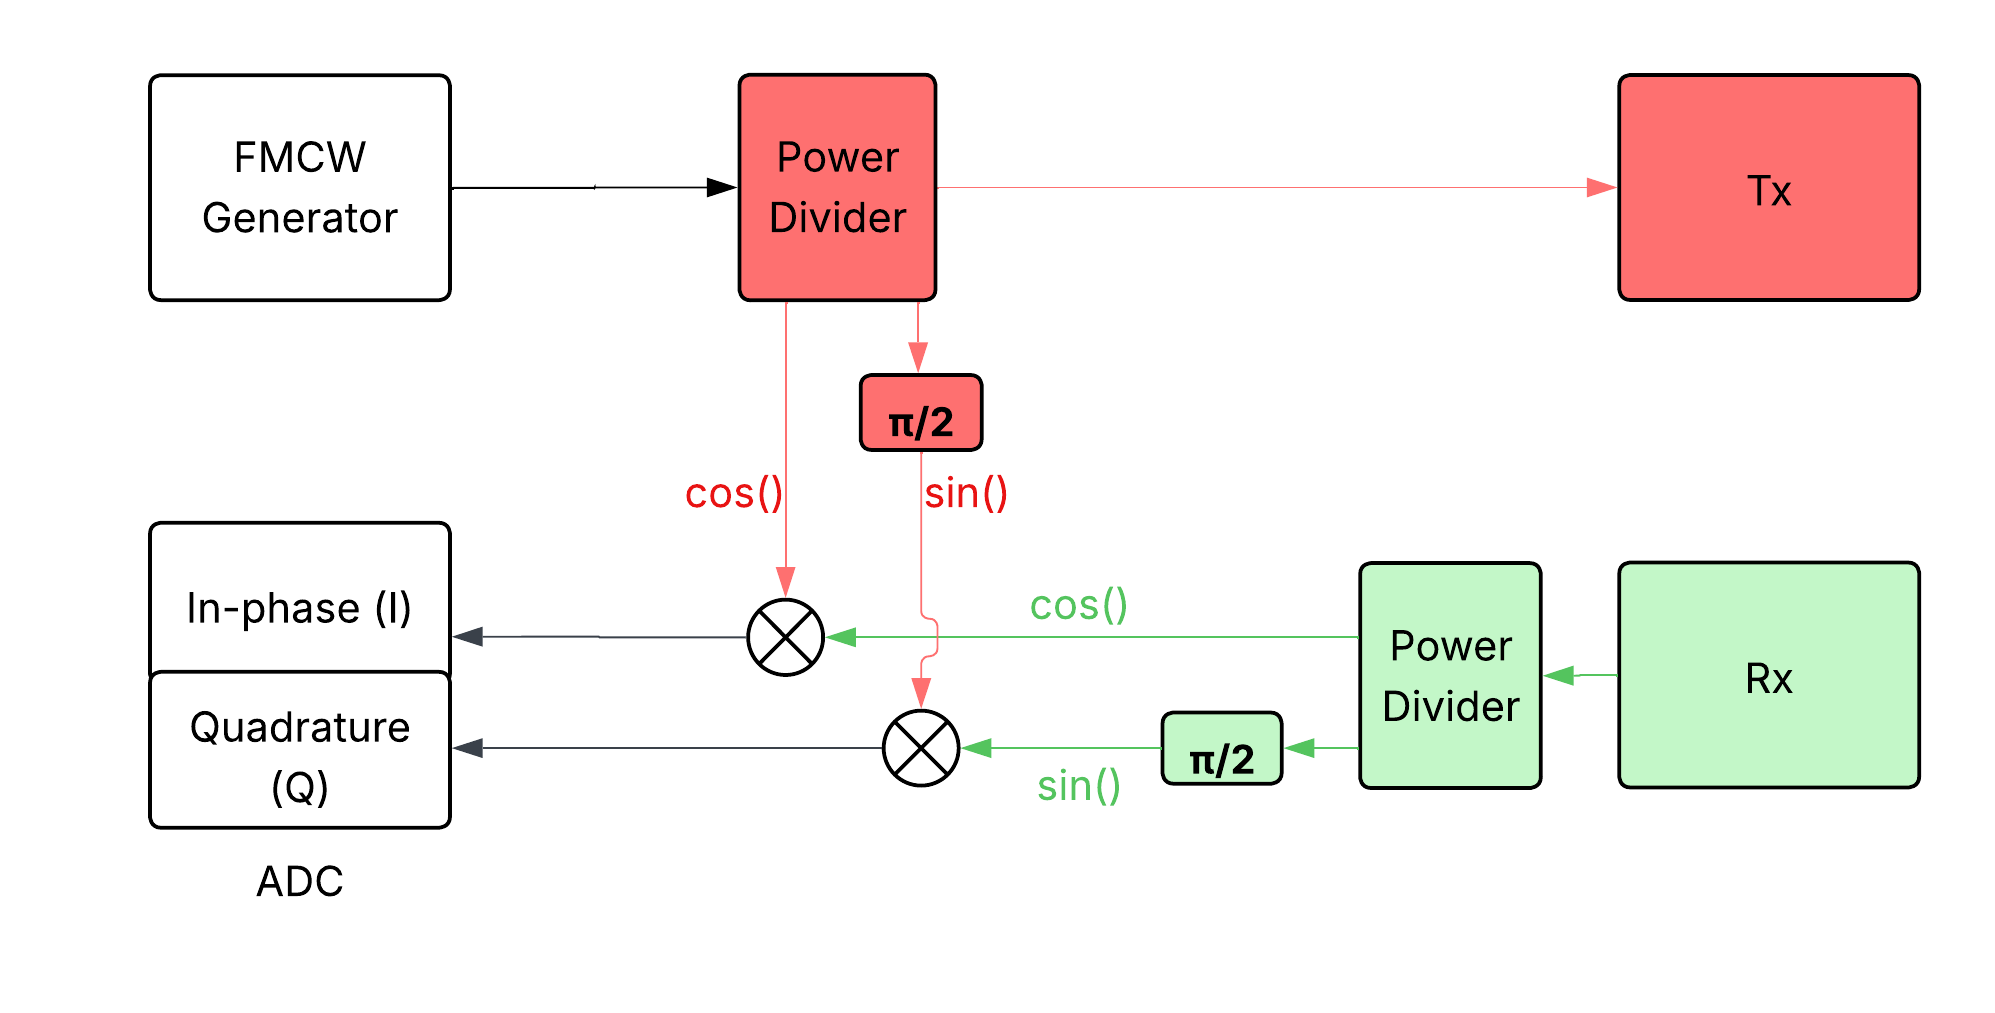
\includegraphics[width=\linewidth]{figs/IQ_demodulation.png}
  \caption{Block diagram of IQ demodulation in FMCW radar. The received echo is mixed with in-phase (I) and quadrature (Q) copies of the transmit chirp and low-pass filtered, producing complex baseband samples that preserve both amplitude and phase for downstream range and angle processing.}
  \label{fig:iq_demod}
\end{figure}

\subsection{IQ Demodulation for Complex Baseband ADC}
\label{sec:supp_iq}

In practice, the RF front-end uses IQ demodulation as shown in Fig.~\ref{fig:iq_demod}. A single real mixer would fold the symmetric RF sidebands at $\pm f_{\mathrm{IF}}$ onto the same baseband frequencies, effectively aliasing positive and negative beat frequencies onto the same baseband bins. IQ mixing instead produces a complex-valued baseband signal with a one-sided spectrum, keeping positive and negative frequencies separated, improving SNR, and yielding an unambiguous mapping between beat frequency and range~\cite{270463, alizadeh2019remote}.

A copy of the transmit chirp is routed to the local-oscillator (LO) ports of two mixers: one LO branch uses a cosine (in-phase, I) and the other a $90^\circ$-shifted sine (quadrature, Q). The received RF signal is applied to the RF port of both mixers, and each output is low-pass filtered and digitized, yielding
\begin{align}
    I(t) &\propto \cos\!\big(2\pi f_{\mathrm{IF}} t + \phi(t)\big),\\
    Q(t) &\propto \sin\!\big(2\pi f_{\mathrm{IF}} t + \phi(t)\big).
\end{align}
Interpreting these as the real and imaginary parts of a single complex baseband beat signal,
\begin{equation}
    m(t) = I(t) + j\,Q(t),
\end{equation}
is equivalent to multiplying the received RF with a complex LO and discarding the image band.

To make this analytic form explicit, we write the transmitted and received chirps using Euler’s formula following~\cite{270463}:
\begin{align}
    s(t) &= A_s \exp\!\big(j (2\pi f_c t + \pi K t^2)\big),\\
    u(t) &= A_r \exp\!\big(j [2\pi f_c (t-\tau) + \pi K (t-\tau)^2]\big).
\end{align}
Ideal IQ demodulation corresponds to mixing the received signal with the complex conjugate of the transmit signal:
\begin{equation}
    m(t) = u(t)\,s^*(t).
\end{equation}
Using the phase difference between $u(t)$ and $s(t)$, this simplifies to
\begin{align}
    m(t) 
    &= A_s A_r \exp\!\left(
        j \left[ 2\pi K \tau\, t + 2\pi f_c \tau - \pi K \tau^2 \right]
    \right) \\
    &\approx A_m \exp\!\left(
        j \left[ 2\pi f_{\mathrm{IF}} t + \phi(t) \right]
    \right),
    \label{eq:complex_baseband_continuous}
\end{align}
where again $f_{\mathrm{IF}} = K \tau = 2 K d/c$ and $\phi(t) \approx 4\pi d/\lambda$.

Finally, the ADC samples this complex baseband signal at rate $f_s$, producing discrete-time IQ data
\begin{equation}
    m[n] \approx A_m 
    \exp\!\left(
        j \left[ 2\pi f_{\mathrm{IF}} \frac{n}{f_s} + \phi[n] \right]
    \right),
    \label{eq:adc_samples}
\end{equation}
where $n$ indexes fast-time samples within a chirp and $\phi[n]$ encodes the path-length-dependent phase (and any slow motion) at the $n$-th sample. These complex ADC samples are the starting point for our subsequent MIMO imaging formulation.


\subsection{TDM MIMO for 2D and 3D Imaging}
\label{sec:tdm_mimo_imaging}

The complex ADC samples in~\eqref{eq:adc_samples} describe a single transmit--receive pair observing a single target. Modern mmWave sensors instead use multiple transmit (TX) and receive (RX) antennas arranged in an array and operate them in time-division multiplexing (TDM) mode to synthesize a larger \emph{virtual} aperture. This enables 2D and 3D spatial imaging via discrete Fourier transforms over carefully chosen dimensions of the ADC data cube, as described by~\cite{9658500}.

\paragraph{TDM MIMO data cube.}
Let $N_\text{TX}$ and $N_\text{RX}$ denote the number of physical transmitters and receivers, $N_\text{chirp}$ the number of chirps in a frame, and $N_\text{s}$ the number of fast-time ADC samples per chirp. In a TDM sequence, only one TX is active at a time. Each chirp slot is assigned to a particular transmitter, cycling through all $N_\text{TX}$ elements.

For TX element $i \in \{0,\dots,N_\text{TX}-1\}$, RX element $j \in \{0,\dots,N_\text{RX}-1\}$, chirp index $\ell \in \{0,\dots,N_\text{chirp}-1\}$, and fast-time sample index $n \in \{0,\dots,N_\text{s}-1\}$, the sampled complex beat signal can be written as
\begin{equation}
    m_{ij}[\ell,n] \approx A_{ij}[\ell]\,
    \exp\!\left(
        j\left[
            2\pi f_{\mathrm{IF}} \frac{n}{f_s}
            + \phi_{ij}[\ell]
        \right]
    \right),
    \label{eq:tdm_mimo_sample}
\end{equation}
where $f_s$~is the ADC sampling rate, $A_{ij}[\ell]$~captures path loss and BSDF/antenna gains, and the phase~$\phi_{ij}[\ell]$ contains the range phase~$4\pi d/c$ plus offsets from TX/RX array geometry and slow motion across chirps.

Stacking all $(i,j,\ell,n)$ produces a four-dimensional data block. For convenience, the TX/RX indices are often flattened into a \emph{virtual} antenna index $v \in \{0,\dots,N_\text{V}-1\}$ with $N_\text{V} = N_\text{TX} N_\text{RX}$, giving $m_v[\ell,n]$.

\paragraph{Range FFT (fast-time).}
The first processing step is a 1D FFT along fast time $n$ for each virtual channel $v$ and chirp $\ell$, which converts beat frequency to range. Before the FFT, a Hann window $w_\text{R}[n]$ is applied in fast time to suppress spectral leakage and sidelobes:
\begin{equation}
    M_v[\ell,k]
    =
    \sum_{n=0}^{N_\text{s}-1}
        w_\text{R}[n]\,
        m_v[\ell,n]\,
        \exp\!\left(
            -j \frac{2\pi}{N_\text{s}} k n
        \right),
    \label{eq:range_fft}
\end{equation}
$\qquad k = 0,\dots,N_\text{s}-1.$ Each frequency bin $k$ corresponds to a range
\begin{equation}
    R_k = \frac{c\,k}{2B},
    \label{eq:range_bin}
\end{equation}
so the magnitude $\lvert M_v[\ell,k]\rvert$ encodes the reflectivity at range $R_k$ observed by virtual channel $v$. Range estimation is therefore driven primarily by the \emph{amplitude} of the fast-time FFT, while the complex phase of $M_v[\ell,k]$ is carried forward for angle processing.

\paragraph{Angle-of-arrival from virtual array phase.}
At a fixed range bin $k$, a far-field target arriving from direction $(\theta,\varphi)$ (azimuth and elevation) produces nearly identical amplitudes across the virtual aperture but a systematic phase ramp tied to the projection of the direction vector onto each element’s position. For a 1D linear virtual array along $x$ with inter-element spacing $d_x$, the phase at element $v$ satisfies
\begin{equation}
    \phi_v(k) \approx \phi_0(k) 
    + \frac{2\pi}{\lambda}\, x_v \sin\theta,
\end{equation}
where $x_v$ is the $x$-coordinate of virtual element $v$. Taking a DFT over the virtual array index therefore steers beams in angle:
\begin{align}
\widetilde{M}[k,n_\theta]
&=
\sum_{v=0}^{N_\mathrm{V}-1}
    w_\mathrm{AZ}[v]\,
    \Big(
        \frac{1}{N_\text{chirp}}
        \sum_{\ell=0}^{N_\text{chirp}-1}
            M_v[\ell,k]
    \Big)
    \nonumber\\
&\quad\times
    \exp\!\left(
        -j \frac{2\pi}{N_\mathrm{V}} n_\theta v
    \right),
\label{eq:azimuth_fft}
\end{align}

where $w_\text{AZ}[v]$ is a spatial (e.g., Hann) window applied across the virtual aperture to reduce angular sidelobes. The bin index $n_\theta$ maps to azimuth angle via the usual array steering relation,
\begin{equation}
    \theta_{n_\theta}
    \approx \sin^{-1}\!\left(
        \frac{\lambda}{N_\text{V} d_x}\, n_\theta
    \right),
\end{equation}
assuming half-wavelength spacing and small-angle approximation. Here, the \emph{relative phase} of $M_v[\ell,k]$ across $v$ is what encodes direction-of-arrival. The FFT over $v$ converts this phase gradient into an angular spectrum. The result $\lvert \widetilde{M}[k,n_\theta]\rvert$ is a 2D range--azimuth (RA) map.

When the physical TX and RX antennas are arranged in a 2D grid, TDM MIMO produces a 2D virtual array indexed by $(v_x,v_z)$ along horizontal and vertical baselines with spacings $d_x$ and $d_z$. After the range FFT, two consecutive spatial FFTs over $v_x$ and $v_z$ yield a 3D range--azimuth--elevation (RAE) cube:
\begin{align}
\widetilde{M}_x[k,n_\theta,v_z]
&=
\sum_{v_x} w_\text{AZ}[v_x]\,
    \bar{M}[k,v_x,v_z]\,
    \nonumber\\
&\quad\times
    \exp\!\left(
        -j \frac{2\pi}{N_x} n_\theta v_x
    \right),
\label{eq:mx_fft}
\\[0.3em]
\widetilde{M}_{xz}[k,n_\theta,n_\phi]
&=
\sum_{v_z} w_\text{EL}[v_z]\,
    \widetilde{M}_x[k,n_\theta,v_z]\,
    \nonumber\\
&\quad\times
    \exp\!\left(
        -j \frac{2\pi}{N_z} n_\phi v_z
    \right).
\label{eq:mxz_fft}
\end{align}

with $N_x$ and $N_z$ the number of virtual elements in azimuth and elevation, and $w_\text{EL}[v_z]$ an elevation window. The indices $(n_\theta,n_\phi)$ map to azimuth and elevation angles via the corresponding steering relations. In our pipeline, these RA/RAE tensors are obtained by applying Hann windows in each FFT dimension to suppress sidelobes and then using the magnitudes $\lvert \widetilde{M} \rvert$ for downstream 2D/3D imaging.

\paragraph{Slow-time (Doppler) dimension.}
For moving targets, the chirp index $\ell$ carries an additional phase term proportional to radial velocity. A further FFT along $\ell$ recovers Doppler frequency and yields range-Doppler-angle cubes commonly used in automotive tracking. In this work, we do not model the motion of the radar via an additional Doppler phase term, nor do we apply a Doppler FFT over all chirps. Instead, our inverse renderer assumes static scenes even though the data was collected from a moving platform, and we therefore partially attribute residual differences between rendered and ground-truth ADC to this simplification. For 2D/3D spatial imaging, we apply only the fast-time FFT for range and the virtual-array FFTs for azimuth and elevation, all acting on the same complex baseband ADC samples in~\eqref{eq:tdm_mimo_sample}.

\subsection{Bistatic Radar Equation: From RCS to MC Estimator}
\label{sec:supp_mc_derivation}

This section provides the full derivation of the Monte Carlo estimator used in the main paper (Eq.~3). We follow an RX-centric formulation where rays are traced from the receiver.

\paragraph{Area-domain form.}
For a single TX--RX pair observing a surface point $\mathbf{x}$ with normal $\mathbf{n}$, distances $d_t = \|\mathbf{x} - \mathbf{x}_{tx}\|$ and $d_r = \|\mathbf{x}_{rx} - \mathbf{x}\|$, and unit directions $\boldsymbol{\omega}_t$ (toward TX) and $\boldsymbol{\omega}_r$ (toward RX), the differential received power is:
\begin{equation}
    P_r(\mathbf{x})
    =
    V \cdot P_t\,
    \frac{G_t(\boldsymbol{\omega}_t)\,G_r(\boldsymbol{\omega}_r)\,\lambda^2}{(4\pi)^2\, d_t^2\, d_r^2}
    \;
    f(\boldsymbol{\omega}_t, \mathbf{x}, \boldsymbol{\omega}_r)\;
    c_t\, c_r\, dA_x,
    \label{eq:supp_radar_area}
\end{equation}
where $V \in \{0,1\}$ is visibility, $G_t$, $G_r$ are directional antenna gains, $f$ is the surface BSDF, and $c_t = \max(0, \mathbf{n} \cdot \boldsymbol{\omega}_t)$, $c_r = \max(0, \mathbf{n} \cdot \boldsymbol{\omega}_r)$ are cosine factors. This relates to the standard bistatic radar equation (main paper Eq.~1) by replacing the point-target RCS $\sigma$ with a distributed BSDF: $\sigma = 4\pi \int f \, c_t \, c_r \, dA$.

\paragraph{Change of variables to receiver solid angle.}
When sampling directions at the receiver, we express the surface integral in receiver solid angle $d\omega_r$ via:
\begin{equation}
    d\omega_r = \frac{c_r}{d_r^2}\, dA_x
    \qquad \Longleftrightarrow \qquad
    c_r\,dA_x = d_r^2\, d\omega_r.
    \label{eq:supp_omega_area}
\end{equation}
Substituting into~\eqref{eq:supp_radar_area}, the factor $c_r\,dA_x / d_r^2$ becomes $d\omega_r$, so both $d_r^2$ and $c_r$ are absorbed:
\begin{equation}
    P_r
    =
    \frac{P_t\,\lambda^2}{(4\pi)^2}
    \int_{\Omega_{rx}}
    \frac{
    G_t(\boldsymbol{\omega}_t)\,G_r(\boldsymbol{\omega}_r)\,
    f(\boldsymbol{\omega}_t, \mathbf{x}, \boldsymbol{\omega}_r)\,
    c_t\, V
    }{
    d_t^2
    }
    \, d\omega_r.
    \label{eq:supp_solid_angle}
\end{equation}

\paragraph{Single-bounce MC estimator.}
Given $N$ samples $\boldsymbol{\omega}_{r,k} \sim \rho_{rx}(\boldsymbol{\omega})$, the unbiased estimator for~\eqref{eq:supp_solid_angle} is:
\begin{equation}
    \hat{P}_r
    =
    \frac{P_t\,\lambda^2}{(4\pi)^2}\,
    \frac{1}{N}\sum_{k=1}^{N}
    \frac{
    G_t(\boldsymbol{\omega}_{t,k})\,G_r(\boldsymbol{\omega}_{r,k})\,c_{t,k}\,f_k\,V_k
    }{
    d_{t,k}^2\,\rho_{rx}(\boldsymbol{\omega}_{r,k})
    }.
    \label{eq:supp_mc_single}
\end{equation}

\paragraph{Multi-bounce generalization.}
For a path $x_{rx} \to x_1 \to x_2 \to \cdots \to x_D \to x_{tx}$ of depth $D$, we sample the initial direction at the receiver with PDF $\rho_{rx}$, each intermediate direction with PDF $\rho_\ell$, and connect deterministically to the transmitter from $x_D$. Each surface-to-surface segment contributes a geometric coupling factor $\mathcal{G}_\ell = c_{\ell \to \ell+1}\, c_{\ell+1 \to \ell} / d_{\ell,\ell+1}^2$. The unbiased $D$-bounce estimator is:
\begin{equation}
    \hat{P}_r^{(D)}
    =
    \frac{P_t\,\lambda^2}{(4\pi)^2}\,
    \frac{1}{N}\sum_{k=1}^{N}
    \left[
    \frac{G_r(\boldsymbol{\omega}_{r,k})}{\rho_{rx}(\boldsymbol{\omega}_{r,k})}
    \prod_{\ell=1}^{D-1}
    \frac{f_\ell\, \mathcal{G}_\ell}{\rho_\ell}
    \;\cdot\;
    \frac{G_t(\boldsymbol{\omega}_{t,k})\, c_{D \to tx}\, f_D}{d_{D,tx}^2}
    \cdot V_k
    \right].
    \label{eq:supp_mc_multi}
\end{equation}
The single-bounce case ($D=1$) reduces to~\eqref{eq:supp_mc_single} when the product is empty. We use Russian roulette for unbiased path termination at configurable depth.

\subsection{From Received Power to ADC Counts}
\label{sec:supp_power_to_adc}

The MC estimator in~\eqref{eq:supp_mc_single}--\eqref{eq:supp_mc_multi} yields the received power $\hat{P}_r$ in Watts for each path. In the main paper (Eq.~\ref{eq:path_adc}), this is written as the complex amplitude $a_{ij}^{(p)}$ that ``aggregates MC throughput.'' Here we make explicit how received power is converted to ADC counts in the renderer.

\paragraph{E-field to voltage.}
In a matched $Z_0$-ohm system ($Z_0 = 50\,\Omega$ for standard RF), the received electric field amplitude relates to power via
\begin{equation}
    V = \sqrt{P_r \cdot Z_0},
    \label{eq:supp_voltage}
\end{equation}
where $V$ is the baseband voltage at the ADC input.

\paragraph{Voltage to ADC counts.}
The ADC digitizes the baseband voltage with a full-scale range corresponding to $2^{15} = 32{,}768$ counts for a 16-bit signed converter. The conversion is
\begin{equation}
    s_\text{ADC} = V \cdot \text{ADC}_\text{fs},
    \label{eq:supp_adc_scale}
\end{equation}
where $\text{ADC}_\text{fs} = 32{,}768$. Combining~\eqref{eq:supp_voltage} and~\eqref{eq:supp_adc_scale}, the end-to-end scale factor from $\sqrt{\text{Watts}}$ to ADC counts is
\begin{equation}
    \alpha_\text{ADC} = \sqrt{Z_0} \cdot \text{ADC}_\text{fs} = \sqrt{50} \times 32{,}768 \approx 231{,}660.
    \label{eq:supp_adc_combined}
\end{equation}

\paragraph{Per-path ADC amplitude.}
For a single path $p$ from TX $i$ to surface point $\mathbf{x}$ to RX $j$, the complex ADC amplitude in Eq.~\ref{eq:path_adc} is therefore
\begin{equation}
    a_{ij}^{(p)} = \alpha_\text{ADC} \cdot G_\text{rx}' \cdot \sqrt{L_\text{ant} \cdot \hat{P}_{r,k}^{(p)}},
    \label{eq:supp_adc_amplitude}
\end{equation}
where $\hat{P}_{r,k}^{(p)}$ is the MC power estimate for path $p$ from~\eqref{eq:supp_mc_single} or~\eqref{eq:supp_mc_multi}, $L_\text{ant}$ is the round-trip antenna/PCB loss (linear), and $G_\text{rx}' = 10^{(G_\text{rx,dB} - \Delta_\text{dBFS})/20}$ is the effective programmable receiver gain after accounting for the dBm-to-dBFS offset $\Delta_\text{dBFS} = 13$\,dBm. With $G_\text{rx,dB} = 30$\,dB and $L_\text{ant} = -4$\,dB, the effective gains are $G_\text{rx}' \approx 7.08$ and $\sqrt{L_\text{ant}} \approx 0.63$.

\paragraph{Hardware parameters.}
Table~\ref{tab:hardware_params} lists the radar hardware constants used in the forward model, following TI AWR2243 specifications.

\begin{table}[t]
\centering
\caption{Radar hardware parameters used in the forward model.}
\label{tab:hardware_params}
\begin{tabular}{lcc}
\toprule
\textbf{Parameter} & \textbf{Symbol} & \textbf{Value} \\
\midrule
Transmit power & $P_t$ & 13\,dBm \\
Programmable RX gain & $G_\text{rx}$ & 30\,dB \\
Antenna/PCB loss & $L_\text{ant}$ & 4\,dB \\
System impedance & $Z_0$ & 50\,$\Omega$ \\
ADC full scale & $\text{ADC}_\text{fs}$ & 32,768 (16-bit signed) \\
dBm-to-dBFS offset & -- & 13\,dBm \\
\bottomrule
\end{tabular}
\end{table}

\paragraph{Note on the $(4\pi)^2$ vs.\ $(4\pi)^3$ factor.}
The standard bistatic radar equation (main paper Eq.~\ref{eq:radar_bistatic}) uses a $(4\pi)^3$ denominator because it includes a point-target RCS $\sigma$. In the RX-centric solid-angle formulation of~\eqref{eq:supp_solid_angle}, the change of variables from surface area to receiver solid angle (Eq.~\ref{eq:supp_omega_area}) absorbs one factor of $d_r^2$ and the cosine $c_r$, effectively replacing the third $4\pi$ factor. The MC estimator therefore uses $(4\pi)^2$ in the denominator, which is consistent with the distributed-BSDF formulation.

\subsection{Range and Angular Resolution}
\label{sec:supp_range_angle_resolution}

This section describes the resolution terms as they relate to hardware parameters~\cite{9658500}, which in turn informs inverse problems in radar imaging such as super-resolution (along range, azimuth and/or elevation) as well as 2D-to-3D lifting~\cite{li2023azimuth}.

\paragraph{Range resolution and windowing.}
For a linear FMCW chirp with effective sweep bandwidth $B$, the
beat-frequency spacing after a $K$-point range FFT corresponds to a
range-bin spacing
\begin{equation}
    \Delta R \approx \frac{c}{2B},
\end{equation}
so two point targets at the same angle are resolvable in range if they
are separated by more than $\Delta R$~\cite{9658500}. 

\paragraph{Virtual aperture and angular resolution.}
After range processing, we form a virtual array by concatenating all
$N_\text{TX} N_\text{RX}$ transmitter–receiver pairs. For a given range
bin, the complex entry associated with virtual element $(p,q)$ on the
2D grid (azimuth index $p$, elevation index $q$) can be modeled as
\begin{equation}
    s_{pq} \propto 
    \exp\!\Big(
        j \, \tfrac{2\pi}{\lambda} 
        \big( p\,d_x \sin\theta \cos\phi + q\,d_z \sin\phi \big)
    \Big),
\end{equation}
where $(\theta,\phi)$ are azimuth and elevation, $d_x$ and $d_z$ are
element spacings along $x$ and $z$, and $\lambda$ is the carrier
wavelength. For a uniform linear array of $N$ elements with spacing
$d=\lambda/2$, the broadside 3\,dB angular resolution scales
approximately as
\begin{equation}
    \Delta \theta \approx \frac{\lambda}{N d}
    \approx \frac{2}{N} \;\text{radians},
\end{equation}
with an analogous expression for elevation resolution $\Delta\phi$ when
a vertical aperture is present~\cite{9658500}.

\paragraph{TI MMWCAS for training vs.\ dense virtual array for inference.}
The TI MMWCAS RF-EVM board used for training realizes a time-division
MIMO configuration with at most $N_\theta \approx 86$ virtual
elements arranged predominantly along a single azimuth dimension and a
very sparse sampling in elevation. Assuming $\lambda/2$ spacing, the
ideal azimuth resolution at broadside is on the order of
\begin{equation}
    \Delta \theta \approx \frac{2}{N_\theta}
    \approx 0.023~\text{rad} \approx 1.3^\circ,
\end{equation}
before windowing. Elevation resolution is minimal due to the sparse vertical baseline.

For 3D scene reconstruction at test time, we synthesize a dense $100 \times 100$ virtual aperture inspired by the Rohde \& Schwarz QAR50~\cite{rs_qar}, with
$\lambda/2$ spacing along both azimuth and elevation (see
Fig.~\ref{fig:antenna_layouts}, right). In this case,
$N_\theta = N_\phi = 100$, yielding near-isotropic
degree-level resolution:
\begin{equation}
    \Delta \theta \approx 
    \Delta \phi \approx
    \frac{2}{100} \approx 0.02~\text{rad} \approx 1.1^\circ
\end{equation}
for a rectangular aperture. More importantly, the 2D virtual grid avoids the strong
anisotropy of a 1D azimuth-only array: the point-spread function is
approximately separable and well conditioned in both angular
directions, enabling true 3D range–azimuth–elevation imaging via a
3D FFT on the ADC data cube.



\subsection{Polar-to-Cartesian Conversion}
\label{sec:supp_polar_to_cartesian}

After TDM MIMO processing, the radar data is expressed in spherical (range--angle) coordinates. For visualization and comparison with camera/LiDAR, we convert RA/RAE maps to Cartesian grids.

\paragraph{2D Range–Azimuth.}
The range–azimuth FFT yields a complex map $M[k,n_\theta]$. We use its magnitude
\[
    A[k,n_\theta] = |M[k,n_\theta]|
\]
as samples of $A(R_k,\theta_{n_\theta})$, where $R_k = k\,\Delta R$ with $\Delta R$ from~\eqref{eq:range_bin}. Azimuth bins are obtained from a uniform grid in spatial frequency:
\[
    u_{n_\theta} = \frac{2n_\theta - N_\theta}{N_\theta}, 
    \qquad
    \theta_{n_\theta} = \arcsin(u_{n_\theta}),
\]
corresponding to the array FFT sampling in $\sin\theta$.

We build a Cartesian grid $(x_i,y_j) \in [-W,W]\times[0,D]$ with $D = N_R \Delta R$ and $W = D/2$, and associate each polar sample with planar coordinates
\[
    x_{k,n_\theta} = R_k \sin\theta_{n_\theta}, \qquad
    y_{k,n_\theta} = R_k \cos\theta_{n_\theta} - b_R,
\]
where $b_R$ is a small range bias. The scattered samples $(x_{k,n_\theta},y_{k,n_\theta},A(R_k,\theta_{n_\theta}))$ are then resampled onto the regular 2D grid $(x_i,y_j)$ via bilinear interpolation, yielding a Cartesian RA image $A_\text{Cart}(y_j,x_i)$.

\paragraph{3D RAE processing.}
For the 3D case, the range--azimuth--elevation FFT produces $M[k,n_\theta,n_\phi]$ with magnitudes
\[
    A[k,n_\theta,n_\phi] = |M[k,n_\theta,n_\phi]|
    = A(R_k,\theta_{n_\theta},\phi_{n_\phi}).
\]
Azimuth and elevation angles are obtained from spatial frequencies $u_\theta,u_\phi \in [-1,1]$ via
\[
    \theta_{n_\theta} = \arcsin(u_{\theta,n_\theta}), \qquad
    \phi_{n_\phi} = \arcsin(u_{\phi,n_\phi}),
\]
consistent with the virtual-aperture steering relations in Sec.~\ref{sec:supp_range_angle_resolution}.

Each triple $(R_k,\theta_{n_\theta},\phi_{n_\phi})$ is mapped to Cartesian coordinates in our radar-centric frame:
\[
\begin{aligned}
    x_{k,n_\theta,n_\phi} &= R_k \cos\phi_{n_\phi}\,\sin\theta_{n_\theta}, \\
    y_{k,n_\theta,n_\phi} &= R_k \cos\phi_{n_\phi}\,\cos\theta_{n_\theta} - b_R, \\
    z_{k,n_\theta,n_\phi} &= R_k \sin\phi_{n_\phi}.
\end{aligned}
\]
We then resample these points onto a regular voxel grid $(x_i,y_j,z_\ell)$ using trilinear interpolation, producing a Cartesian volume $A_\text{Cart}(x_i,y_j,z_\ell)$ that can be rendered as 3D heatmaps, iso-surfaces, or point clouds aligned with camera/LiDAR coordinates.
\section{Implementation Details}
\label{sec:supp_implementation}

\subsection{Input Data Format and Pre-Processing}
\label{sec:supp_preprocessing}

Our method operates on synchronized radar and LiDAR data from the ColoRadar dataset~\cite{kramer2022coloradar}. We extract cascaded FMCW radar ADC data for the target frame, applying both phase and frequency calibration to the raw ADC samples before transposing to the format $(N_C, N_{Rx}, N_{Tx}, N_{ADC})$, where $N_C$ is the number of chirps, $N_{Rx}$ and $N_{Tx}$ are the receiver and transmitter counts, and $N_{ADC}$ is the ADC sample count. To construct the 3D scene geometry, we aggregate approximately 50 LiDAR frames centered temporally around the radar observation, transforming each frame to world coordinates using ground truth vehicle poses and cropping to the radar field-of-view. We remove exact duplicates and points coinciding with sensor positions, yielding a fused point cloud typically containing 100,000--500,000 points. Surface normals are estimated using GPU-accelerated radius search (FAISS) with a 0.1m neighborhood radius: for each point, we compute the covariance matrix of its neighbors and extract the eigenvector corresponding to the
smallest eigenvalue, then orient normals toward the nearest LiDAR sensor position to ensure consistent outward-facing orientation.

Finally, we reconstruct a triangle mesh from the oriented point cloud using screened Poisson surface reconstruction~\cite{kazhdan2006poisson}. We set the octree depth to 8, point weight to 1.0, and apply aggressive surface trimming with threshold 8.0 to remove spurious geometry far from the input points. This produces a clean mesh (typically 200,000--800,000 triangles) suitable for our differentiable ray tracing renderer. All processed data (calibrated ADC samples, individual LiDAR frames, aggregated point clouds with normals, and reconstructed meshes) are saved in standardized formats (NumPy arrays for radar/LiDAR data, PLY for meshes) for reproducibility. For each scene, JSON files specify the radar array geometry, waveform parameters, and calibrated extrinsics for rendering.

\subsection{LiDAR-Radar Coarse-to-Fine Alignment}
\label{sec:supp_alignment}

Due to residual calibration errors between the LiDAR and radar coordinate frames, we perform an automated coarse-to-fine extrinsic alignment procedure before training. This aligns the LiDAR-derived mesh with the radar observations by optimizing over a 4-DoF transformation: range translation $\Delta r$, azimuth translation $\Delta\theta$, and rotations around the elevation and azimuth axes ($\phi_\text{el}$, $\phi_\text{az}$).

\paragraph{Coarse grid search (GPU-accelerated).}
We first perform a coarse grid search over the 4D parameter space. For each candidate transformation, we project the LiDAR point cloud into radar range-azimuth (RA) coordinates using the transformed sensor pose, apply antenna pattern weighting, and accumulate intensity-weighted histograms into the RA grid. The resulting synthetic LiDAR-derived RA map is compared against the ground truth radar RA map using Pearson correlation as the objective:
\begin{equation}
    \rho = \frac{\sum_{i,j} (L_{ij} - \bar{L})(R_{ij} - \bar{R})}{\sqrt{\sum_{i,j}(L_{ij} - \bar{L})^2}\sqrt{\sum_{i,j}(R_{ij} - \bar{R})^2}},
\end{equation}
where $L$ and $R$ are the min-max normalized LiDAR and radar RA maps. The grid search uses 5--7 steps per dimension with typical search ranges: $\Delta r \in [-3, 3]$~m, $\Delta\theta \in [-15^\circ, 15^\circ]$, $\phi_\text{el}, \phi_\text{az} \in [-10^\circ, 10^\circ]$. GPU acceleration via CuPy enables evaluation of $\sim$2500 grid points in under 2 seconds.

\paragraph{Fine optimization.}
Starting from the best coarse grid point, we refine the alignment using Nelder-Mead optimization (unconstrained, 200 iterations). The fine stage converges to sub-degree angular and sub-centimeter translational precision. Final metrics typically achieve correlation $\rho > 0.7$ between aligned LiDAR and radar RA maps, with the optimized extrinsics saved to a JSON configuration file for subsequent training.

% \subsection{Inverse Renderer}

\subsection{Amplitude-Only Optimization and Gradient Stabilization}
\label{sec:phase_sensitivity_loss_landscape}

Each ADC sample is a coherent sum of multi-bounce phasors $w_i \cdot e^{j\phi_i}$, where $w_i$ is the real-valued amplitude (BSDF, antenna gains, geometric factors) and $\phi_i \propto d_i / \lambda$ encodes the round-trip path length. At mmWave frequencies ($\lambda \approx 4$\,mm), a sub-millimeter change in path length induces an $\mathcal{O}(1)$ change in phase, making phase gradients with respect to geometry or pose extremely noisy: micrometer-scale parameter perturbations flip phasors between constructive and destructive interference, producing spiky, oscillatory gradients that dominate and destabilize optimization~\cite{chen2025invertwin}.

\paragraph{Amplitude-only gradient propagation.}
To avoid this instability, we \emph{detach} the phase trigonometric terms from the automatic differentiation graph. Each path's contribution to the ADC is written as:
\begin{equation}
    s_\text{real} = w \cdot \overline{\cos(\phi)}, \qquad
    s_\text{imag} = w \cdot \overline{\sin(\phi)},
\end{equation}
where $\overline{(\cdot)}$ denotes a stop-gradient operation. Gradients therefore flow from the loss through the amplitude~$w$ to material parameters, normals, and antenna patterns, but the gradient path through phase $\to$ delay $\to$ geometry is blocked. This design choice means our optimizer cannot directly exploit path-length information---a limitation we discuss further in Sec.~\ref{sec:limitations} (Sec.~\ref{sec:lim_amplitude_only})---but yields smooth, well-behaved gradients that converge reliably. In our experiments, amplitude-only gradients produce more stable convergence and slightly higher training correlation than full phase+amplitude gradients.

\paragraph{Amplitude-gradient challenges.}
Even with phase detached, amplitude gradients present challenges due to (i) Monte Carlo variance from stochastic path sampling, which introduces per-iteration gradient noise, and (ii) large dynamic range across parameter groups: material parameters (437,604 degrees of freedom) produce dense gradients with moderate magnitude, while antenna patterns and vertex normals have fewer parameters but can exhibit sporadic large gradients from individual high-energy paths. These effects motivate per-parameter-group gradient clipping to prevent any single group from dominating the Adam update.

\paragraph{Per-parameter group gradient clipping.}
For each parameter group $\theta_k$, we compute the RMS gradient norm:
\begin{equation}
    \|\nabla_{\theta_k} \mathcal{L}\|_{\text{RMS}} = \sqrt{\frac{1}{|\theta_k|} \sum_{i \in \theta_k} (\nabla_{\theta_k^i} \mathcal{L})^2},
\end{equation}
where $|\theta_k|$ is the total number of scalar parameters in group $k$. If this norm exceeds a predefined threshold $\tau_k$, we rescale all gradients in the group by
\begin{equation}
    \nabla_{\theta_k} \mathcal{L} \leftarrow \frac{\tau_k}{\|\nabla_{\theta_k} \mathcal{L}\|_{\text{RMS}}} \, \nabla_{\theta_k} \mathcal{L}.
\end{equation}
This operation \emph{only clips down} large gradients; when $\|\nabla_{\theta_k} \mathcal{L}\|_{\text{RMS}} \leq \tau_k$, no scaling is applied.

We set parameter-specific thresholds informed by empirical analysis of gradient magnitudes during training:
\begin{itemize}
    \item $\tau_{\text{materials}} = 1.0$ for per-vertex material parameters,
    \item $\tau_{\text{pose\_rotation}} = \tau_{\text{pose\_translation}} = 0.5$ for radar pose parameters,
    \item $\tau_{\text{normals}} = 0.5$ for per-vertex normals,
    \item $\tau_{\text{patterns}} = 1.0$ for antenna beam patterns,
    \item $\tau_{\text{vertex\_positions}} = 0.1$ for vertex positions.
\end{itemize}
Combined with learning-rate warmup and per-parameter learning rates, gradient clipping improves convergence stability across all parameter groups.

\subsection{Training Details}
\label{sec:supp_training}

We optimize scene parameters via end-to-end automatic differentiation using our differentiable FMCW radar renderer. The training procedure optimizes per-vertex ITU physics material parameters ($\varepsilon_r'$, $\varepsilon_r''$, $\sigma_h$, $l_c$, $\tau$, slab thickness $d$), vertex normals, and antenna beam patterns while keeping vertex positions and radar pose fixed (Sec.~\ref{sec:optimization}). We train for 500 iterations using 1,500 reservoir hit samples per RX antenna element, with Specular Manifold Sampling (SMS) for specular paths and free-space diffraction (FSD) BSDF~\cite{steinberg2024fsd} for edge diffraction.

The primary loss is min--max normalized range--azimuth L2 (Eq.~\ref{eq:ra_loss}), with Laplacian regularization ($\lambda_\text{geom} = 0.3$) for geometric smoothness when normals are optimized (vertex positions are kept fixed). All $\sqrt{\cdot}$ operations in the AD pipeline use epsilon guards ($10^{-20}$) to prevent infinite gradients at zero-crossings.

\begin{table}[ht!]
\centering
\caption{Training hyperparameters used for all seven scenes. Renderer and optimizer settings are shared across scenes; only input data paths differ.}
\label{tab:training_hyperparams}
\small
\setlength{\tabcolsep}{4pt}
\begin{tabular}{lc}
\toprule
\textbf{Hyperparameter} & \textbf{Value} \\
\midrule
\multicolumn{2}{l}{\emph{Renderer}} \\
\quad Polarization & Vertical \\
\quad Max bounces & 3 \\
\quad Reservoir hits per RX & 1{,}500 \\
\quad Hemisphere sampling & Cosine \\
\quad SMS (specular manifold) & Enabled (20 iter, tol $10^{-5}$) \\
\quad Edge diffraction (FSD) & Enabled \\
\quad Russian roulette & Start bounce 3, $p=0.5$ \\
\midrule
\multicolumn{2}{l}{\emph{Optimizer}} \\
\quad Iterations & 500 \\
\quad Optimizer & Adam ($\beta_1\!=\!0.9$, $\beta_2\!=\!0.999$) \\
\quad LR warmup & $0.3{\times} \to 1{\times}$ over 5 iterations \\
\quad Material parameterization & Per-vertex, 6 ITU params \\
\quad Initial material & Concrete (ITU-R P.2040) \\
\quad Error-map initialization & Enabled \\
\quad Pattern mode & Shared (1 TX + 1 RX pattern) \\
\midrule
\multicolumn{2}{l}{\emph{Optimized parameters}} \\
\quad Materials & \checkmark \\
\quad Vertex normals & \checkmark \\
\quad Antenna patterns & \checkmark \\
\quad Pose (rotation / translation) & Frozen \\
\quad Vertex positions & Frozen \\
\midrule
\multicolumn{2}{l}{\emph{Loss}} \\
\quad Primary loss & Log-compressed RA L2 \\
\quad Log epsilon & $10^{-6}$ \\
\quad Laplacian regularization & $\lambda_\text{geom} = 0.3$ \\
\quad Phase gradient & Detached (amplitude only) \\
\bottomrule
\end{tabular}
\end{table}

\paragraph{Per-group learning rates and gradient clipping.}
Learning rates are set per parameter group: materials $= 0.5$, pose rotation $= 5 \times 10^{-3}$, pose translation $= 5 \times 10^{-4}$, vertex normals $= 0.01$, antenna patterns $= 0.05$, vertex positions $= 5 \times 10^{-4}$. We apply per-group RMS gradient clipping (materials$=1.0$, pose rotation$=0.5$, pose translation$=0.5$, normals$=0.5$, patterns$=1.0$, vertex positions$=0.1$) to stabilize training against MC variance and inter-group dynamic range differences (Sec.~\ref{sec:phase_sensitivity_loss_landscape}). A linear learning rate warmup (0.3$\times$ to 1$\times$ over 5 iterations) prevents initial divergence. Post-step constraints clamp pose translation to $\pm\lambda/2$ and rotation to $\pm 2^{\circ}$ per iteration.

Within the material parameter group, per-column learning rate scales further modulate the Adam update for each of the six material parameters ($\varepsilon_r'$: 0.3, $\varepsilon_r''$: 0.5, $\sigma_h$: 0.3, $l_c$: 0.3, $\tau$: 0.5, $d$: 0.1). These scales reflect the relative sensitivity of the loss to each parameter; in particular, slab thickness~$d$ receives the smallest scale (0.1) because its effect on slab Fresnel resonance is highly nonlinear.

\paragraph{Material parameterization.}
Each vertex stores 6 ITU physics parameters reparameterized for unconstrained optimization. Table~\ref{tab:material_reparam} summarizes the transforms and bounds.

\begin{table}[ht!]
\centering
\caption{Material parameter reparameterization. The optimizer operates in unconstrained space $x$; each parameter is mapped to a bounded physical value via the listed transform. Clamp bounds are applied before the exponential to prevent overflow.}
\label{tab:material_reparam}
\begin{tabular}{lccc}
\toprule
\textbf{Parameter} & \textbf{Transform} & \textbf{Physical range} & \textbf{Clamp} \\
\midrule
$\varepsilon_r'$ & $1.5 + 8.5\,\sigma(x)$ & $[1.5, 10]$ & -- \\
$\varepsilon_r''$ & $e^{\text{clamp}(x)}$ & $[10^{-3}, 9{\times}10^{6}]$ & $[-7, 16]$ \\
$\sigma_h$ (m) & $e^{\text{clamp}(x)}$ & $[10^{-7}, 10^{-3}]$ & $[-16, -7]$ \\
$l_c$ (m) & $e^{\text{clamp}(x)}$ & $[5{\times}10^{-4}, 0.1]$ & $[-7.6, -2.3]$ \\
$\tau$ & $0.05 + 0.9\,\sigma(x)$ & $[0.05, 0.95]$ & -- \\
$d$ (m) & $e^{\text{clamp}(x)}$ & $[10^{-3}, 0.3]$ & $[-7, -1.2]$ \\
\bottomrule
\end{tabular}
\end{table}

Initialization uses ITU-R P.2040 reference values for common materials: concrete ($\varepsilon_r' = 5.31$, $\varepsilon_r'' = 0.29$), glass ($\varepsilon_r' = 6.27$, $\varepsilon_r'' = 0.15$), and metal ($\varepsilon_r' = 1.0$, $\varepsilon_r'' = 10^7$) at 77~GHz. For a typical scene with 72,934 vertices, this yields 437,604 material degrees of freedom.

\paragraph{Error-map-driven material initialization.}
Before gradient-based training begins, we optionally run a single non-differentiable forward pass with the default material initialization and compare the rendered RA map against the ground truth. Triangles whose rendered intensity significantly exceeds the ground truth (over-reflecting phantom triangles) are identified via a per-triangle error map, and their initial material parameters are pre-adjusted (increasing imaginary permittivity $\varepsilon_r''$ and roughness $\sigma_h$) to reduce their reflected energy before optimization. This prevents the optimizer from wasting early iterations correcting large phantom contributions inherited from imperfect mesh reconstruction.

\paragraph{Antenna pattern mode.}
All TX and RX elements share a single learnable beam pattern (``shared'' mode). The pattern is initialized from reference MMWCAS element patterns and jointly optimized with material and normal parameters during training. This reduces the pattern degrees of freedom from $N_\text{TX} + N_\text{RX}$ independent patterns to a single shared pattern, which is appropriate given the uniform element design of the TI MMWCAS board.

Training each scene requires approximately 10--15 minutes on a single NVIDIA RTX~4090 GPU (24\,GB). Checkpoints are saved every 50 iterations, and the iteration with the lowest training loss is saved separately.

\paragraph{Amplitude-only gradient propagation.}
As detailed in Sec.~\ref{sec:phase_sensitivity_loss_landscape}, we detach the phase trigonometric terms from the AD graph and propagate gradients only through the real-valued amplitude~$w$ of each phasor. This blocks the noisy phase$\to$delay$\to$geometry gradient path while preserving smooth, stable amplitude gradients to material parameters, normals, and antenna patterns.

\subsection{Inference Details}
\label{sec:supp_inference}

\paragraph{Dense Array Configuration}
To generate dense radar data while maintaining consistency with the MMWCAS sensor board frame, we first create dense antenna array configurations using a uniform virtual antenna array generator. Starting from the original MMWCAS config (12 TX × 16 RX), we generate a dense array with 100 TX $\times$ 100 RX elements arranged in a two-column TX and two-row RX pattern as shown in Figure~\ref{fig:antenna_layouts} (right). The dense antennas are mapped to the same board plane as the original MMWCAS array using PCA-based board frame extraction to recover the exact horizontal, vertical, and boresight axes from the antenna positions. All dense antennas are positioned with half-wavelength ($\lambda /2 = 1.97 $mm at 76 GHz) spacing and collectively translated so the dense array's geometric center exactly matches the original MMWCAS board center, preserving both position and orientation. 
\paragraph{Dense Array ADC Generation}
For ADC generation, we employ batched rendering with 100 TX-RX pairs per batch to manage GPU memory when processing the 10,000-element MIMO array. We trace 200 reservoir hit samples per RX element with reflection enabled. Since the goal at test time is 3D scene reconstruction, we follow~\cite{kung2025radarsplat} and use single-bounce propagation (max path depth = 1, i.e., one surface interaction per path) at test time with this dense radar array. The forward model uses antenna pattern-weighted importance sampling and loads all trained scene parameters (materials, normals, and learned antenna beam patterns) from optimization checkpoints. The renderer accumulates all path contributions (diffuse reflection, specular reflection via SMS, and edge diffraction via FSD) into a single coherent complex ADC tensor of shape (100 TX, 100 RX, 256 ADC samples, 2). Rendering a single ADC frame for the dense radar array takes approximately 6\,seconds on an RTX~4090.


\subsection{Post-Processing Details}
\label{sec:supp_postprocess}

% \paragraph{Dense Array ADC to 3D Radar Point Cloud.}
Once the dense radar array ADC data is generated, we apply full FMCW processing: range FFT produces a 3D complex cube, virtual array mapping creates a $100 \times 100 \times 256$ tensor, followed by azimuth and elevation FFTs yielding a $127 \times 127 \times 256$ Range-Azimuth-Elevation (RAE) cube. We extract the board frame (azimuth, range, elevation axes) from antenna positions, which is then used to align the local RAE cube to the global 3D Cartesian coordinate frame. In summary, for the radar point cloud extraction, we: (1) compute magnitude RAE, (2) threshold at the 99.9th percentile, (3) convert to metric 3D coordinates, and (4) apply rigid transformation (translation + rotation) to align with scene ground truth.

% \paragraph{Evaluation Metrics Against LiDAR Ground Truth.}
% Following the precedent set by prior work~\cite{kung2025radarsplat}, we evaluate a percentile-thresholded radar point cloud against the original LiDAR ground truth with radar-guided filtering. For LiDAR preprocessing, we: (1) filter by antenna beam pattern using the dense radar array antenna beam pattern TX/RX 0dB beam limits in azimuth and elevation, (2) project remaining LiDAR points onto the radar polar voxel grid, and (3) retain only points where radar has normalized intensity $\geq 0.1$, effectively restricting evaluation to regions with radar returns. For distance-based occupancy metrics, we build KD-trees for both point clouds, compute nearest neighbor distances, and classify points as matched if within $\tau = 0.5$~m threshold to calculate precision, recall, specificity, and accuracy. For geometric fidelity, we report RMSE and Chamfer Distance (CD), normalized by scene extent to produce Relative Chamfer Distance (R-CD). The results for each of the four scenes is provided in Table~\ref{tab:3d_occupancy}.

% \paragraph{Performance across scenes varies significantly with scene geometry.}
% Scene 1 achieves strong reconstruction metrics (Precision=0.988, R-CD=0.108) due to multiple surfaces within the radar FOV and especially along the boresight providing multiple significant returns. In contrast, Scenes 3 and 4 show degraded performance (Precision=0.361/0.563, R-CD=0.201/0.192) because these scenes contain primarily open space with only ground planes visible. Given the radar boresight is nearly parallel to the ground plane and surface normals cause specular reflection away from the radar, few returns reach the receivers. This fundamental limitation, combined with our primitive intensity thresholding, results in sparse radar reconstructions for these scenes.


% % \subsection{Benchmark Details}
\section{Additional Results}
\label{sec:supp_qualitative}

This section presents qualitative visualizations and quantitative ablations that complement the main paper's evaluation.
We first visualize the learned parameters, including per-vertex materials (Sec.~\ref{sec:qual_materials}), surface normals (Sec.~\ref{sec:qual_normals}), and antenna beam patterns (Sec.~\ref{sec:qual_beam}),to provide interpretability for the optimized representations.
We then ablate each component of the full model (Sec.~\ref{sec:ablation}) to quantify individual contributions and report runtime breakdowns (Sec.~\ref{sec:runtime}).

\subsection{Material Visualization}
\label{sec:qual_materials}

\begin{figure}[t]
  \centering
  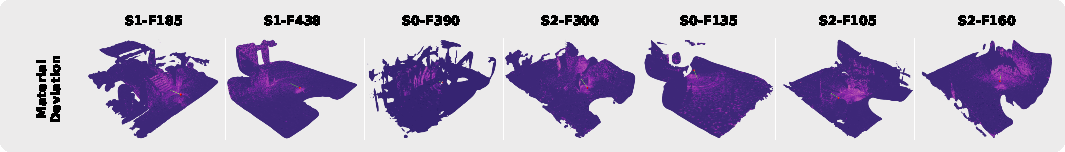
\includegraphics[width=\linewidth]{figs/materials_deviation_v1.pdf}
  \caption{Per-vertex material deviation from ITU-R P.2040 concrete defaults after optimization, shown across all seven scenes. Color encodes the normalized mean deviation across six physics parameters ($\varepsilon_r$, $\varepsilon_i$, $\sigma_h$, $\ell_c$, $\tau$, $d$) using the inferno colormap, where black = zero deviation (unchanged from defaults) and bright yellow = maximum deviation within each parameter's physical range. Log-scale parameters ($\varepsilon_i$, $\sigma_h$, $\ell_c$, $d$) are normalized in log-space; linear parameters ($\varepsilon_r$, $\tau$) in linear-space. Deviations concentrate on radar-visible surfaces and diminish in occluded or shadow regions.}
  \label{fig:3d_material}
\end{figure}

As shown in Fig.~\ref{fig:3d_material}, material deviations are
spatially correlated with radar visibility: surfaces under direct
illumination show the largest updates, while occluded regions retain
their ITU defaults. This pattern is consistent across all seven scenes
despite varying geometry and viewpoints.

\subsection{Surface Normal Visualization}
\label{sec:qual_normals}

\begin{figure}[t]
  \centering
  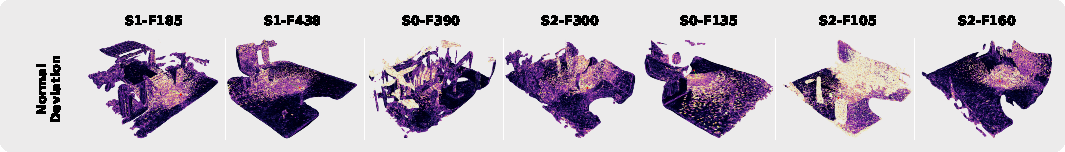
\includegraphics[width=\linewidth]{figs/normals_deviation_v1.pdf}
  \caption{Per-vertex angular deviation between initial (LiDAR-derived) and optimized surface normals across all seven scenes. Color encodes the absolute angle between initial and optimized normal vectors using the inferno colormap, where black = $0^{\circ}$ (no change) and bright yellow = $30^{\circ}$ or greater (clamped at $30^{\circ}$). Larger deviations appear primarily at mesh boundaries and on surfaces with irregular tessellation.}
  \label{fig:normals_deviation}
\end{figure}

\begin{figure}[t]
  \centering
  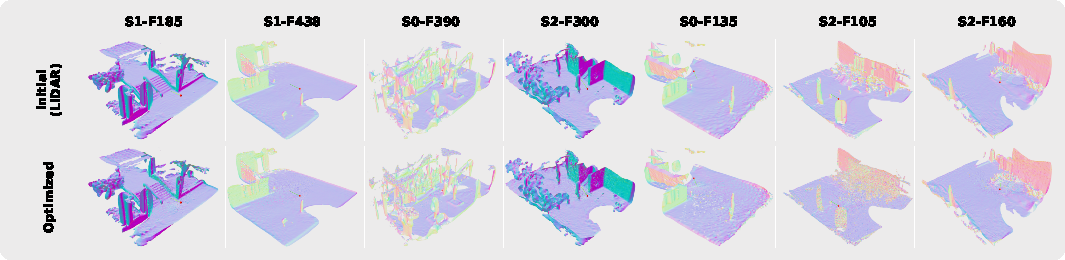
\includegraphics[width=\linewidth]{figs/normals_comparison_v1.pdf}
  \caption{World-space surface normal comparison across all seven scenes. Each vertex is colored by its unit normal direction mapped to RGB (X$\to$R, Y$\to$G, Z$\to$B; value range $[-1,1] \to [0,1]$). Top row (``Initial''): normals computed from the Poisson-reconstructed LiDAR mesh. Bottom row (``Optimized''): normals after joint optimization. Differences between rows show where surface orientations changed during optimization; changes are most apparent at mesh boundaries and on large planar surfaces where Poisson reconstruction artifacts are common.}
  \label{fig:normals}
\end{figure}

Figure~\ref{fig:normals_deviation} shows that angular deviations are spatially concentrated at mesh boundaries, thin structures, and regions with irregular tessellation, all of which are known failure modes of Poisson surface reconstruction from sparse LiDAR returns. Mean angular deviations range from $4^{\circ}$ to $13^{\circ}$ across the seven scenes. Figure~\ref{fig:normals} provides the corresponding world-space normal comparison: large planar regions (walls, ground) remain largely unchanged, while edges and thin features show visible reorientation. This spatial pattern indicates that normal optimization corrects tessellation artifacts rather than overfitting to measurement noise.

\subsection{Antenna Beam Pattern Visualization}
\label{sec:qual_beam}

\begin{figure}[t]
  \centering
  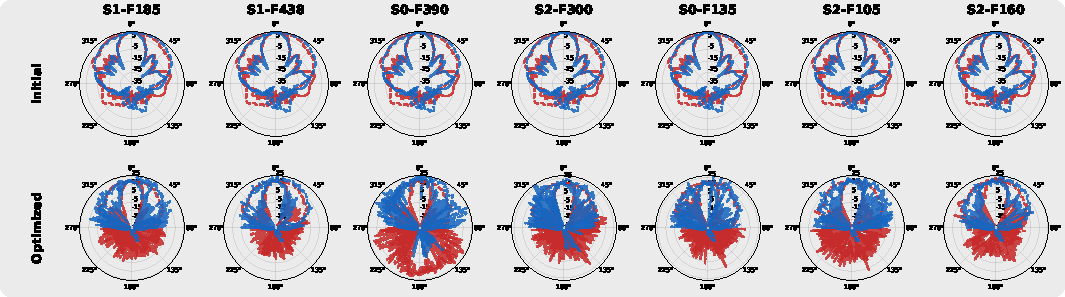
\includegraphics[width=\linewidth]{figs/beam_patterns_comparison_v1.pdf}
  \caption{Antenna beam pattern comparison across all seven scenes (polar plots, dB scale). Each plot shows four curves: TX elevation (red solid), TX azimuth (red dashed), RX elevation (blue solid), and RX azimuth (blue dashed). Top row (``Initial''): reference patterns shared across all scenes. Bottom row (``Optimized''): per-scene optimized patterns. Optimization adjusts main-lobe gain and sidelobe structure to compensate for calibration uncertainty in the reference antenna data. Per-scene variation in the optimized patterns is expected, as each scene compensates independently for calibration uncertainty. All values floored at the initial pattern minimum ($-32$\,dB).}
  \label{fig:beam_patterns}
\end{figure}

As shown in Fig.~\ref{fig:beam_patterns}, the optimized beam patterns retain the main-lobe beamwidths of the initial reference patterns for both TX and RX elements across elevation and azimuth, while adjusting absolute gain levels. Per-scene variation in the optimized patterns reflects independent compensation for calibration uncertainty. The consistent preservation of main-lobe structure across all seven scenes supports the interpretation that pattern optimization primarily refines gain calibration rather than learning physically implausible beam~shapes.


\FloatBarrier
\subsection{Ablation Studies}
\label{sec:ablation}

\begin{table}[ht!]
\caption{Component ablation averaged over seven training scenes (500
iterations each). Each row disables one component from the full mmIR
model. Best per-column in \textbf{bold}.}
\centering
\begin{tabular}{lcccc}
\toprule
\textbf{Configuration} & \textbf{Corr $\uparrow$} & \textbf{PSNR $\uparrow$} & \textbf{SSIM $\uparrow$} & \textbf{RMSE $\downarrow$} \\
\midrule
Full model              & 0.919 & 37.6 & 0.902 & 0.014 \\
\midrule
w/o diffraction         & 0.910 & 37.4 & 0.896 & 0.014 \\
w/o SMS                 & 0.915 & 37.8 & 0.898 & 0.014 \\
w/o multi-bounce        & \textbf{0.936} & \textbf{38.7} & \textbf{0.920} & \textbf{0.012} \\
w/o normal optim.       & 0.919 & 37.4 & 0.909 & 0.014 \\
w/o pattern optim.      & 0.885 & 36.6 & 0.882 & 0.015 \\
w/o error-map init      & 0.909 & 37.4 & 0.895 & 0.014 \\
\bottomrule
\end{tabular}
\label{tab:ablation}
\end{table}


We ablate each component by disabling it from the full model and
retraining on all seven scenes for 500 iterations
(Table~\ref{tab:ablation}). We group ablations into three categories:
rendering transport, optimization targets, and initialization.

\paragraph{Rendering transport.}
Disabling \emph{diffraction} degrades RA correlation ($0.919 \to 0.910$, $-1.0\%$), indicating that edge-diffracted energy
contributes in outdoor scenes with building edges, fences,
and vehicle contours.
%
Disabling \emph{SMS} has a marginal effect on RA metrics
($0.919 \to 0.915$), consistent with the predominantly rough surface
scattering expected at 77\,GHz for outdoor building materials;
SMS primarily benefits scenes with smooth metallic
surfaces (e.g., vehicle panels), which constitute a small fraction of
the total scattering area.
%
Restricting propagation to \emph{single-bounce} slightly improves RA
correlation ($0.919 \to 0.936$) and RMSE
($0.014 \to 0.012$). This suggests that higher-order bounces
introduce Monte Carlo variance at the current sample budget that
slightly degrades metrics, though indirect paths (e.g., ground--wall or
wall--vehicle interactions) contribute measurable energy in the
captured data.

\paragraph{Optimization targets.}
Disabling \emph{antenna pattern optimization} reduces PSNR by
1.0\,dB ($37.6 \to 36.6$) and degrades RA correlation
($0.919 \to 0.885$, $-3.7\%$), indicating that jointly learning beam patterns
compensates for calibration uncertainty in the initial reference antenna
data. As shown in Fig.~\ref{fig:beam_patterns}, the optimized patterns
retain the main-lobe structure and beamwidths of the initial reference
patterns for both TX and RX elements across elevation and azimuth,
indicating that optimization refines gain calibration while preserving
the physical beam structure. The consistent main-lobe preservation
across all seven scenes is consistent with the observation that
disabling pattern optimization primarily degrades PSNR (absolute power
calibration) rather than correlation (spatial structure).
%
Freezing \emph{surface normals} at their LiDAR-derived values has
negligible effect on RA correlation ($0.919 \to 0.919$), while slightly
improving SSIM ($0.902 \to 0.909$). As visualized in
Figs.~\ref{fig:normals_deviation} and~\ref{fig:normals}, normal
optimization concentrates adjustments at mesh boundaries and thin
structures (known failure modes of Poisson surface
reconstruction), with mean angular deviation of $4$--$13^{\circ}$
across scenes, while leaving large planar regions largely unchanged.
This spatial pattern suggests that normal optimization targets
tessellation artifacts rather than overfitting to measurement noise.

\paragraph{Initialization.}
Disabling \emph{error-map initialization} has marginal effect on
final metrics ($0.919 \to 0.909$), indicating that 500 gradient
iterations are sufficient to largely recover from uniform material
initialization. The benefit of error-map seeding is faster early
convergence rather than improved final quality.

\FloatBarrier
\subsection{Runtime}
\label{sec:runtime}

Table~\ref{tab:runtime} reports the runtime breakdown for our pipeline and the Sionna-RT baseline on scene S0F135 ($\sim$72K vertices) using a single NVIDIA RTX 4090 GPU (24\,GB).
Per-scene preprocessing---LiDAR aggregation, Poisson meshing, and radar--LiDAR alignment---is a one-time cost shared by both methods.
During training, our forward render averages 0.65\,s per iteration, roughly $4.5\times$ faster than Sionna-RT's 2.93\,s, owing to our Taichi-based SBR kernel and cached specular-path reuse.
The AD backward pass adds only 0.10\,s.
Including gradient clipping, the Adam optimizer step, and metric computation, the total per-iteration cost is 1.32\,s, enabling 500 iterations in $\sim$11\,min wall-clock time.
At inference, rendering the full dense virtual array (10,000 elements) and computing the RAE FFT takes 6.4\,s per scene.

\begin{table}[ht!]
\centering
\caption{Runtime comparison and breakdown on a single NVIDIA RTX 4090 GPU (24\,GB). Training times are averaged over 500 iterations (mmIR) and 150 iterations (Sionna-RT) on scene S0F135 ($\sim$72K vertices), excluding the first 5 iterations (JIT compilation warmup).}
\label{tab:runtime}
\begin{tabular}{lcc}
\toprule
\textbf{Stage} & \textbf{mmIR (Ours)} & \textbf{Sionna-RT} \\
\midrule
\multicolumn{3}{l}{\emph{Per-scene preprocessing (one-time)}} \\
\quad LiDAR aggregation \& meshing & \multicolumn{2}{c}{144\,s} \\
\quad LiDAR--radar alignment & \multicolumn{2}{c}{2.2\,s} \\
\midrule
\multicolumn{3}{l}{\emph{Training (per iteration, mean $\pm$ std)}} \\
\quad Forward render & 0.65\,s & 2.93\,s \\
\quad AD backward + grad.\ extraction & 0.10\,s & 0.35\,s \\
\quad Grad.\ clipping + optimizer + metrics & 0.57\,s & -- \\
\quad Total per iteration & 1.32 $\pm$ 0.02\,s & 3.28 $\pm$ 0.46\,s \\
\midrule
\multicolumn{3}{l}{\emph{Training (total)}} \\
\quad Total wall-clock & 11.0\,min & 8.2\,min \\
\quad Iterations & 500 & 150 \\
\midrule
\multicolumn{3}{l}{\emph{Inference (one-time per scene)}} \\
\quad Dense array ADC rendering & \multicolumn{2}{c}{6.2\,s} \\
\quad RAE FFT + point cloud & \multicolumn{2}{c}{0.2\,s} \\
\bottomrule
\end{tabular}
\end{table}

\section{Limitations}
\label{sec:limitations}

\subsection{Refraction, Absorption, and Sub-surface Scattering}

Currently, mmIR only models propagation in free space between surface interactions, with interfaces handled by a surface BSDF and diffraction. Transmission into volumes (including glass, plastic, drywall among others), internal attenuation, and sub-surface scattering are not simulated. In effect, any refracted component is absorbed at the first interface. This is reasonable for predominantly metallic and high-contrast scenes, but less accurate for semi-transparent or volumetric media. Supporting these effects would require explicit volumetric permittivity and internal transport via Bidirectional Scattering Distribution Functions (BSDFs), which account for both reflection and transmission.

\subsection{Doppler Phase Term for Moving Radar}

Our FMCW model assumes a static radar pose within each frame and attributes phase only to geometric path length. Ego-motion during a chirp burst introduces an additional Doppler phase term that we do not explicitly model. As a result, mmIR is best matched to quasi-static captures; fast platform motion will induce residual phase errors that cannot be fully absorbed by geometry or material calibration without a time-resolved pose model. Incorporating ego-motion would require a TDM-aware motion model that accounts for platform displacement between successive transmit slots.

\subsection{Dynamic Scenes and Objects}

We optimize a single static mesh with static material parameters to render all ADC measurements. Temporally varying objects (including vehicles, people, vibrating structures) are treated as noise and may appear as blurred or ghosted structure in 3D. To the best of our knowledge, the outdoor scenes chosen from the ColoRadar dataset for our experiments do not feature any moving objects. Accounting for dynamic scenes requires per-frame geometry, deformable models, or an explicit separation of static and dynamic components, which is not currently included and left for future work.

\subsection{Multi-bounce Diffraction}

Diffraction is modeled via the free-space diffraction (FSD) BSDF~\cite{steinberg2024fsd} at single-bounce surface interactions, combined with multi-bounce specular/diffuse reflections. Higher-order diffraction chains (edge--edge, edge--surface--edge) and more detailed grazing-angle behavior are not modeled. Extending to multi-bounce diffraction requires preserving Jones-vector transport along diffracted paths, which the FSD BSDF framework naturally supports. Multi-bounce diffraction may contribute additional energy in highly cluttered or strongly shadowed environments that the current single-bounce model does not capture.

\subsection{Amplitude-Only Gradient Signal}
\label{sec:lim_amplitude_only}

As described in Sec.~\ref{sec:phase_sensitivity_loss_landscape}, each ADC sample contains a phase term $\phi \propto d/\lambda$ that is extremely sensitive to path-length changes: at 77\,GHz ($\lambda \approx 4$\,mm), a sub-millimeter displacement induces an $\mathcal{O}(1)$ change in phase, and a half-wavelength shift produces a full $2\pi$ wrap. In our inverse-rendering setting, small parameter updates change individual path lengths by micrometers, flipping phasor contributions between constructive and destructive interference and producing a highly oscillatory, speckle-like loss landscape with narrow local minima spaced at fractions of the wavelength.

Our default training configuration therefore detaches the phase trigonometric terms $\cos(\phi)$ and $\sin(\phi)$ from the AD graph, propagating gradients only through the amplitude $w$ of each phasor contribution (Sec.~\ref{sec:phase_sensitivity_loss_landscape}). While this improves training stability and convergence, it limits the information available to the optimizer: the loss cannot directly drive parameter updates based on path-length discrepancies. In principle, phase gradients carry complementary geometric information that amplitude alone cannot provide. Enabling full phase+amplitude gradients may benefit future work on joint geometry and material optimization, provided the phase gradient noise can be sufficiently mitigated, for instance via larger sample counts, frequency-dependent phase smoothing, or learned gradient scaling.

\subsection{Mesh Quality Bottleneck}

mmIR is bottlenecked by the quality of the LiDAR-derived mesh used as scene geometry. If the Poisson surface reconstruction introduces artifacts (missing surfaces, incorrect topology, or smoothed-out fine structure), the rendered ADC may diverge from the real measurement despite material or pose optimization. Thin structures (fences, poles, foliage) and regions with sparse LiDAR returns are particularly susceptible to reconstruction error, and may produce \emph{phantom reflectors}: mesh triangles that do not correspond to any real-world surface but still contribute spurious radar returns. Our learnable energy gate $A(\boldsymbol{\omega}_t)$ (Eq.~\ref{eq:bsdf_full}) partially mitigates this: optimization can drive $A \to 0$ for phantom triangles by learning high imaginary permittivity or thin-slab resonance, effectively suppressing their reflected energy.

We further employ an error-map-driven material initialization that identifies over-reflecting triangles (where rendered intensity exceeds ground truth) before gradient-based training and pre-adjusts their roughness and permittivity to reduce phantom contributions. Furthermore, LiDAR ($\lambda \sim 900$~nm) and mmWave radar ($\lambda \sim 4$~mm) interact with surfaces at fundamentally different scales: surfaces that produce strong LiDAR returns (e.g., foliage, thin fabric) may be effectively transparent at mmWave frequencies, while surfaces that are specular at mmWave (e.g., rough concrete) scatter diffusely in LiDAR. The mesh therefore includes surfaces with negligible radar cross-section and may miss structures that are radar-visible but LiDAR-dark. Our learnable energy gate partially compensates by suppressing radar-invisible surfaces, but cannot reconstruct geometry absent from the mesh. Nevertheless, these mechanisms cannot recover surfaces that are missing from the mesh entirely. Mitigating this limitation requires either higher-fidelity meshing pipelines (e.g.,\ neural implicit surfaces, multi-frame aggregation) or jointly optimizing coarse mesh topology during inverse rendering.

\subsection{Sensitivity to Sensor Alignment}

The inverse rendering task is highly sensitive to the LiDAR--radar alignment, both for the cascaded imaging radar used during training and the single-chip radar used for transfer evaluation. Small translational or rotational errors shift rendered paths relative to measured ones, introducing systematic phase errors that material optimization alone cannot absorb. Our coarse-to-fine GPU alignment mitigates gross misalignment but may converge to local optima in scenes with ambiguous geometry (flat surfaces, repetitive structure). This sensitivity is amplified for multi-chip cascade configurations where inter-chip calibration errors compound across the virtual array.



% ---------------------------------------------------------------
% Bibliography (supplement-only references)
\bibliographystyle{splncs04}
\bibliography{supplement_only}

\end{document}
